\documentclass[./main.tex]{subfiles}

\begin{document}
\section{Stacked Hourglass, t-SNE and K-Means Clustering}
In this section the various algorithms and architectures used throughout this thesis is described and explained in details.
\subsection{Stacked Hourglass}
When performing the pose estimation in section \textbf{REFERENCE MANGLER}, we will be implementing and using the \textit{stacked hourglass} described by Newell \textit{et al.} \cite{Newell}. The following description and explanation of the architecture is based on an interpretation of Newell \textit{et al.} \cite{Newell} and Camilla Olsen \cite{Camilla}.

\subsubsection{Reasoning behind using the Stacked Hourglass}
% NOTE: MANGLER MÅSKE AT SKRIVE, AT DER ER SKET MEGET VIDEREBYGNING PÅ SHG SIDEN NEWELL, HVILKET VI KAN BRUGE NÅR VI SKAL BRUGE VORES VIDEN OM MODELLEN TIL AT OPTIMERE DEN.
We have decided to make use of the stacked hourglass described by Newell \textit{et al.}, as it is a intermediate architecture that has shown state-of-the-art results. At the same time the architecture of the network is similar to the architecture of \textit{autoencoders}, making the architecture useful for encoding the data into a lower dimension, which can be useful in section \textbf{REFERENCE MANGLER}, when we will be doing the interpretation of the model.

\subsubsection{The Residual Module}
\begin{figure}[h]
    \centering
    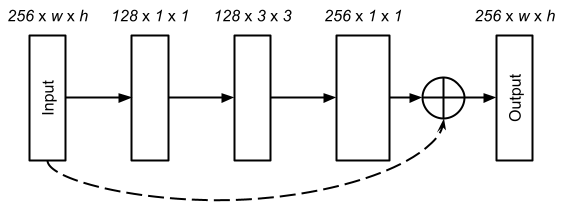
\includegraphics[height = 2 cm]{entities/Residual.png}
    \caption{Visualization of the residual module \cite{Newell}}
    \label{fig:residual}
\end{figure}
\noindent The stacked hourglass makes heavily use of so-called \textit{residual modules}, which is visualized in Figure \ref{fig:residual}. The module works by taking an input, which is sent through a $1 \times 1$ and a $3 \times 3$ convolution, which both return $128$ featuremaps. Then, the $128$ featuremaps are sent through a $1 \times 1$ convolution, which returns $256$ featuremaps. Lastly, element-wise addition is then used to add the $256$ featuremaps to the input of the module, which the model then returns. All convolutions are followed by an acitvation function and are \textit{same convolutions}, meaning the outputted featuremaps are of the same dimensions as the inputted featuremeaps.

\subsubsection{The Hourglass}
\begin{figure}[h]
    \centering
    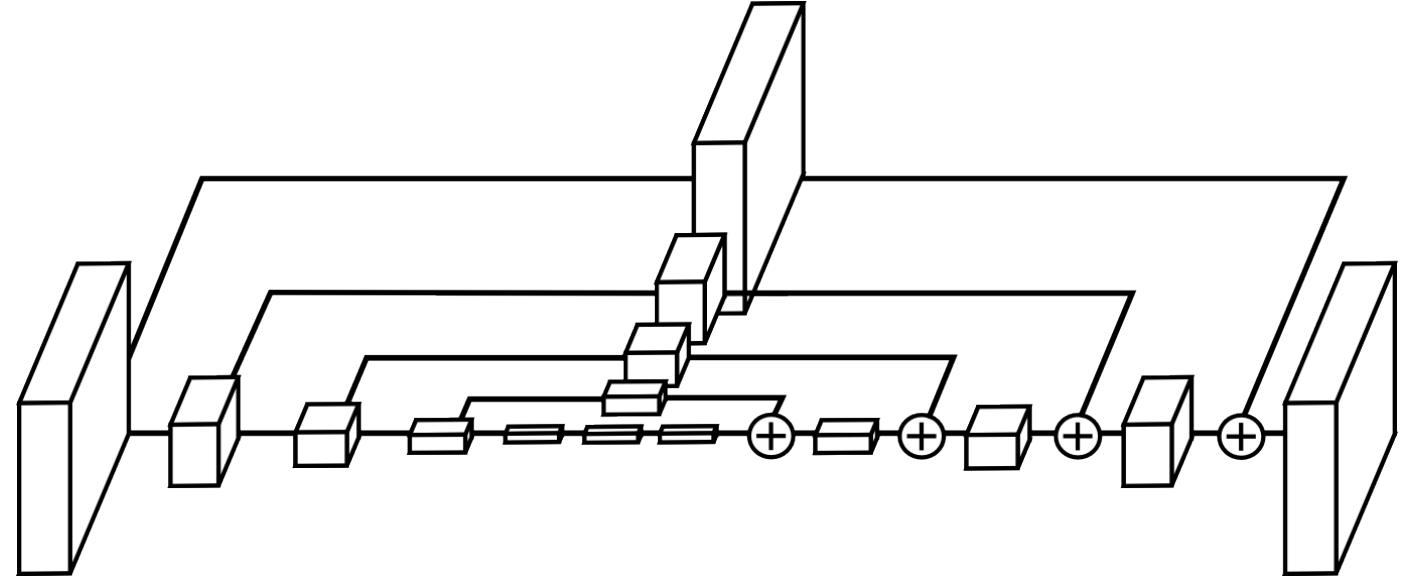
\includegraphics[height = 4 cm]{entities/Hourglass.png}
    \caption{Visualization of a single hourglass \cite{Newell}}
    \label{fig:hourglass}
\end{figure}
\noindent The stacked hourglass consists of hourglasses, where each hourglass is split into an encoder, where the featuremaps is downsampeld, and a decoder, where the featuremaps are upsampled. The hourglass is symmetric, in the sense, that it has an equal amount of downsampling layers in the encoder as there are upsampling layers in the decoder. In Figure \ref{fig:hourglass} a single hourglass han been visualized, where each box is a residual module. The hourglass works by using residuals and max poolings to process features down to a low resolution. Then, nearest neighbor upsampling is used to upsample the featuremaps until the featuremaps have the same dimensions as the input of the hourglass. Before each max pool in the encoder, the network branches off and applies a residual to the feature maps, which are then added element-wise before the corresponding residual in the decoder, which helps to ensure that lost information in the encoder is kept.
Between the encoder and decoder the network has a bottleneck, where no downsampling or upsampling happens, instead only residuals are processing the featuremaps. \\
After the decoder two $1 \times 1$ convolution layers er applied to produce the final predictions of the network.

\subsubsection{The Stacked Hourglass}
\begin{figure}[h]
    \centering
    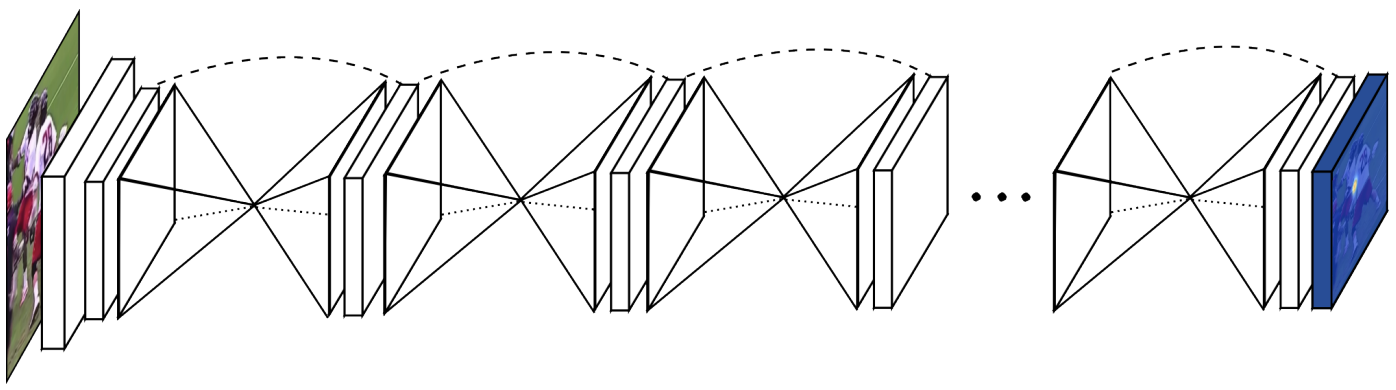
\includegraphics[height = 4 cm]{entities/SHG.png}
    \caption{Visualization of the stacked hourglass \cite{Newell}}
    \label{fig:SHG}
\end{figure}
\noindent The full network is build by stacking multiple hourglasses end-to-end, making the output of one hourglass be the input of the next hourglass, as shown in Figure \ref{fig:SHG}, which makes each hourglass reestimate features of the image. The input of the network is a $256 \times 256$ RGB-image. To lower the memory usage, the network starts off with a $7 \times 7$ convolution layer with stride 2, followed by a residual module and max pooling to bring the resolution down to $64 \times 64$, which is then input to the first hourglass.
By the end the whole network outputs $n$ heatmaps corresponding to the $n$ joints it should predict for a single person. The prediction of a joint is thus the maximum activation of the corresponding heatmap.
% MANGLER AT SKRIVE, AT DER GØRES BRUG AF INTERMEDIATE SUPERVISION, MEN AT DET IKKE ER RELEVANT FOR MIG.

\subsection{t-SNE}
\subsection{K-means Clustering}

\end{document}